% !TeX spellcheck = en_GB
\section{Simulations Experiments}
\subsection{Scenario Calibration}
In order to calibrate the simulator parameters, the following range of values were used:
\begin{itemize}
	\item \textbf{Number of Couples Tx-Rx (N)}: [5, 30]
	\item \textbf{Number of Channels (C)} : [6, 100] (Resource Blocks in LTE for different Frequencies)
	\item \textbf{Mean Inter-arrival Time ($\frac{1}{\lambda}$)}: [125ms, 500ms] (a study was performed in order to choose the mean inter-arrival time that allow us to have meaningful data)   
	\item \textbf{Time-slot duration ($T_{slot}$)}: 5 ms
	\item \textbf{Send Probability (p)}: [0.1, 0.5] 
\end{itemize}

\subsection{Calibration of Warm-Up Period and Simulation duration}
For calibrating the warm-up different simulation were made (with the factors range in the latter paragraph). After various test is clear that the KPI that impacts heavily in the choose of the warmup time is the \textit{Response Time}. We can see the study about the response time in figure \ref{img: warmUp}.
%The worst case in terms of convergence time was encountered with the \textbf{mean throughput} with N = 5, C = 6, $\dfrac{1}{\lambda}$ = 500ms, p = 0.5:
\begin{figure}[H]
	\centering
	\includegraphics[width=\textwidth]{img/warmup.png}
	\caption{Worst Case Warm-up Response Time}
	\label {img: warmUp}
\end{figure}  
%With the \textbf{mean response time} the worst case is the following with N = 5, C = 100, $\dfrac{1}{\lambda}$ = 25ms, p = 0.5:

\noindent\textbf{A warm-up period of 250s was chosen}.\\
For what concerns the simulation duration was made a trade-off between the memory consumption for storing data and the length of the simulation itself. This was done because there are not stochastic elements in the model (like a particular error probability with a low percentage) that will need a particular amount of time to be shown. Obviously the duration has to be greater than the warm-up duration. All things considered, \textbf{a simulation-duration of 5000s was chosen}.

\subsection{Design of Experiments}
\subsubsection{Factorial Analysis $r2^k$ on Throughput}
In order to analyse the contribution of the factors on the throughput performance, we perform a $r2^k$ analysis with $r=5$ and $k=4$ (so we perform $5*2^4 = 80$ experiments). We take into account the following factors:
\begin{itemize}
	\item Number of Couples Tx-Rx: [5, 30] \textbf{(A)}
	\item Number of Channels C : [6, 100] \textbf{(B)}
	\item Send Probability p: [0.2, 0.5] \textbf{(C)}
	\item Mean Inter-arrival Time: [25ms, 500ms] \textbf{(D)}    
\end{itemize}

\noindent The first step is to check the hypothesis, in particular we have to control that the residuals are normal and that its standard deviation is constant (a.k.a. homoskedasticity). For what concerns the normal hypothesis it's possible to see (Figure \ref{img: qqplot_throughput}) that the QQ plot of residuals vs normal show a linear tendency and so the hypothesis is verified.

\noindent For the homoskedasticity we have a QQ plot residuals vs predicted response and we can see (Figure \ref{img: homoskedasticity_throughput}) that indeed there is a trend, however the errors (y axis) are two order of magnitude below the predicted response (x axis) and so we can ignore trends and state that the homoskedasticity hypothesis is respected.

\begin{figure}[H]
	\centering
	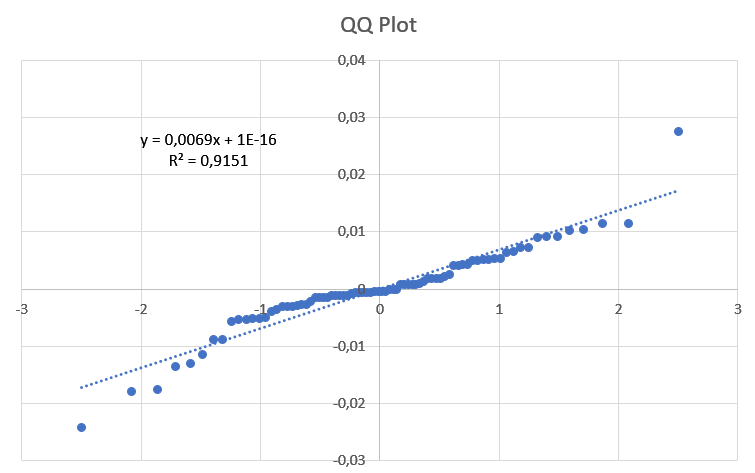
\includegraphics[width=0.8\textwidth]{img/QQplot_2kr_throughput.png}
	\caption{QQ Plot for testing the normal hypothesis}
	\label {img: qqplot_throughput}
\end{figure}

\begin{figure}[H]
	\centering
	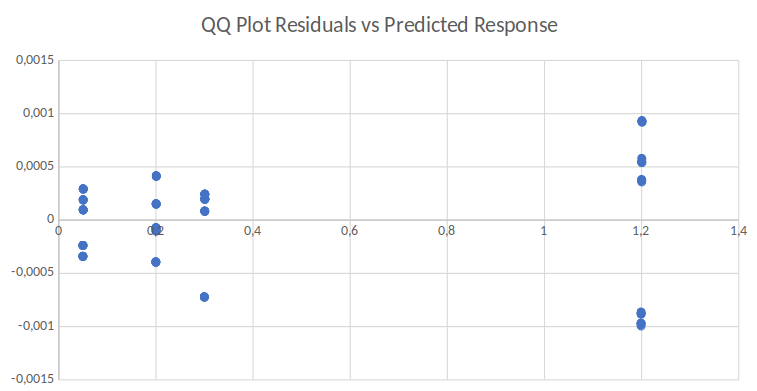
\includegraphics[width=0.8\textwidth]{img/homoskedasticity_2kr_throughput.png}
	\caption{QQ Plot for testing homoskedasticity}
	\label {img: homoskedasticity_throughput}
\end{figure}

\noindent Now we can analyse the obtained results. The most relevant ones are the following (the other factors have an impact on the variability that is very low, below $5\%$, and so they are non relevant):

\begin{itemize}
	\item \textbf{Number of Couples}
	
	\noindent It has a positive impact on throughput, in particular $qi = [0,6689; 0,6701]$\footnote{This and the following are 95\% confidence interval} and it accounts for the 19,67\% of the variability. This means that the higher the number of couples the higher the throughput. In fact with more transmitters we have more packets and so we have an higher throughput.
	 
	\item \textbf{Mean Inter-Arrival Time}
	
	\noindent It has a negative impact: $qi = [-0,8899; -0,8887]$ and it accounts for the 34,71\% of the varibility. Thus we can say that the higher the mean inter-arrival time, the lower the throughput. This happens due to the fact that when we increase the mean inter-arrival time it's more likely that a transmitter have an empty buffer and so it has no packets to transmit, then the throughput decreases. 
	
	\item \textbf{Jointly Effect of Number of Couples and Mean Inter-Arrival Time}
	
	\noindent The jointly effect of the above factors accounts for the 13,07\% of the variability and it has a negative impact ($qi = [-0,5463; -0,5451]$). This because the effect of the mean inter-arrival time is greater with respect to the one of the number of couples, so if both increase then the throughput decreases. Indeed, if we have an higher number of transmitters, but we have the most of them which have an empty buffer (due to the previously explained phenomenon caused by the increasing of the mean inter-arrival time), then the throughput decreases because there are too few packets to transmit.
\end{itemize}

\subsection{Result Analysis}

\begin{figure}[H]
	\centering
	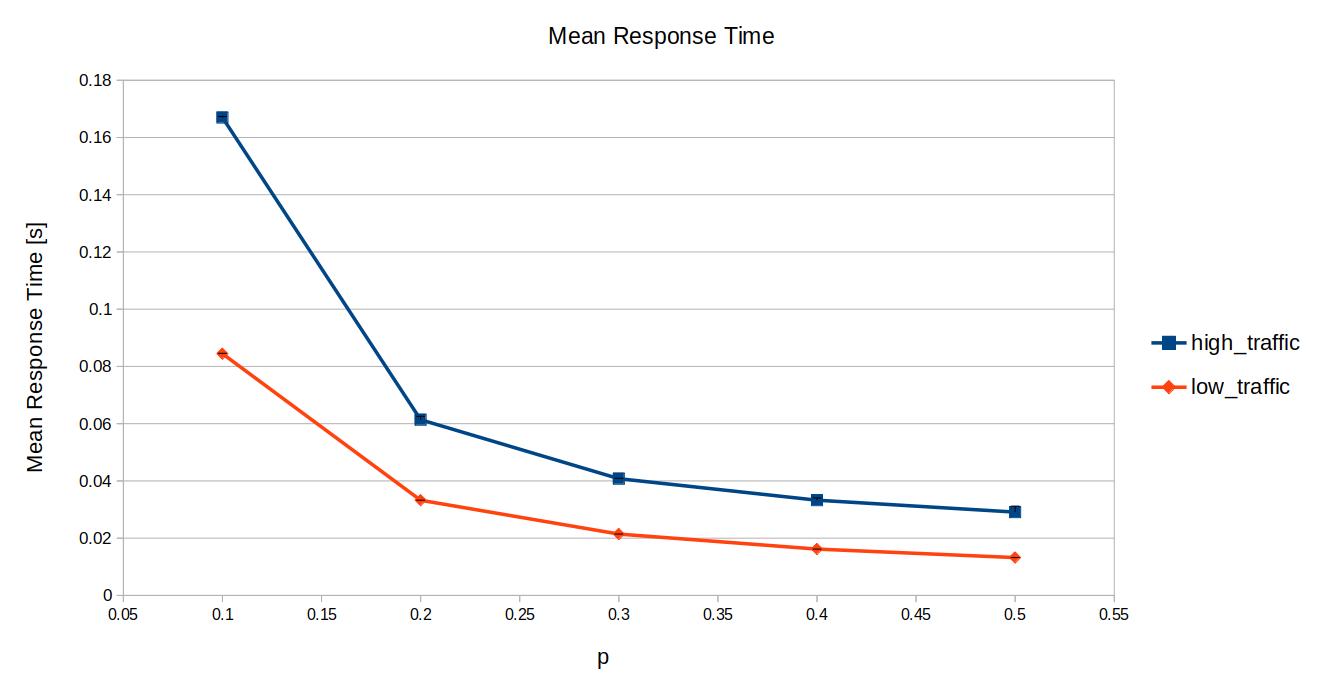
\includegraphics[width=\textwidth]{img/MeanResponseTimeInsight.png}
	\caption{Insight 1}
\end{figure}
\begin{figure}[H]
	\centering
	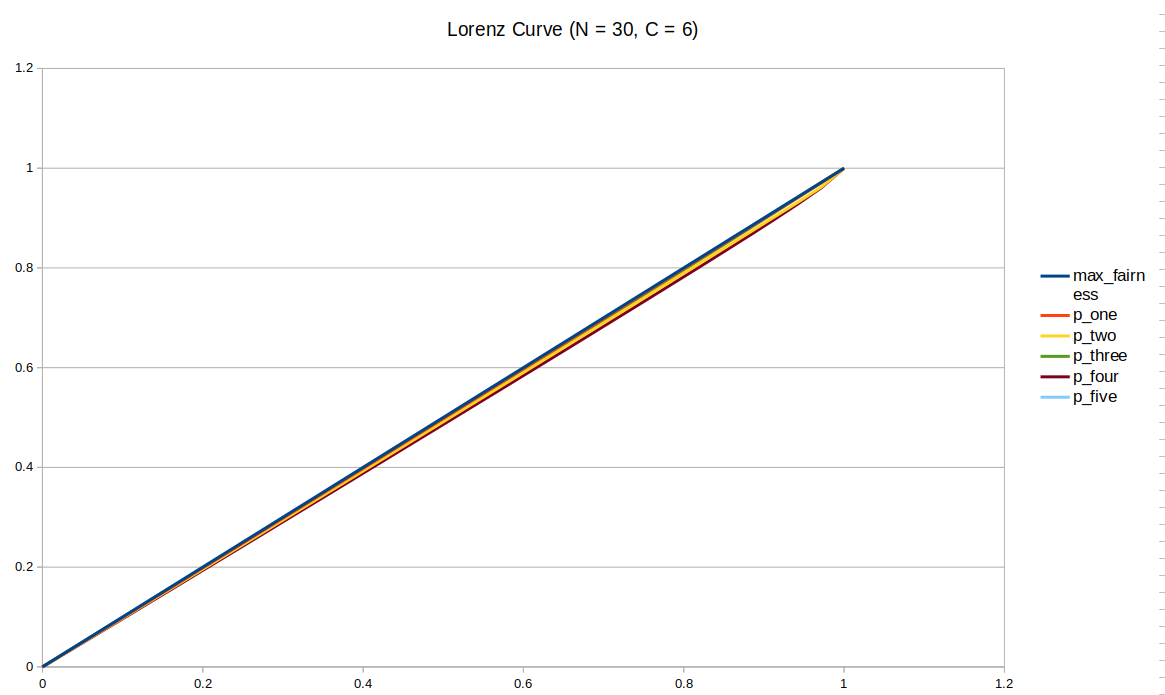
\includegraphics[width=\textwidth]{img/LorenzHighTraffic.png}
	\caption{Insight 2}
\end{figure}
\begin{figure}[H]
	\centering
	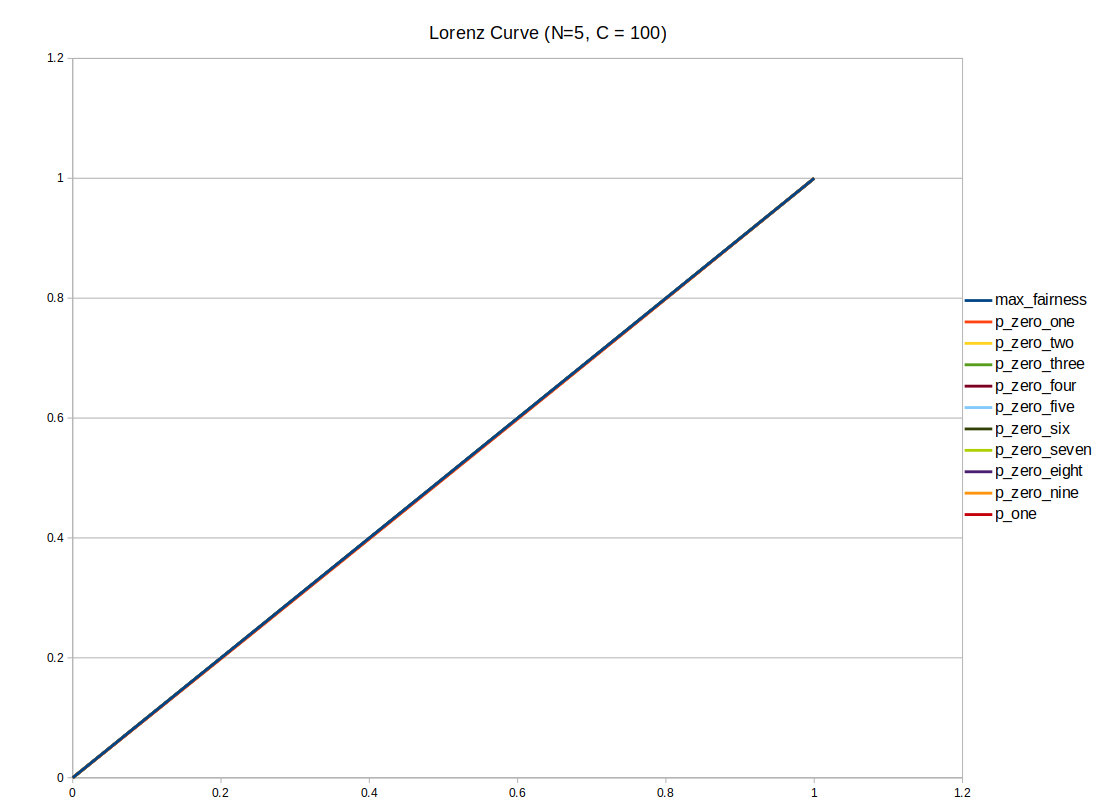
\includegraphics[width=\textwidth]{img/LorenzLowTraffic.png}
	\caption{Insight 3}
\end{figure}